\documentclass{article}%scrartd
\usepackage{graphicx}
\usepackage{amsmath}
\begin{document}
\section{Phasenangeschnittenen Strom messen}
Im Labor soll nun ein phasenangeschnittener Strom gemessen und mit der DFT untersucht werden.
Dazu wird der Dimmer auf dem "Lampenbrett" verwendet.
\subsection{Versuchsaufbau}
Allgemein gilt: Um Strom zu messen muss man ein Amperemeter in Reihe mit der Last schalten. Daher muss auch hier der Stromwandler aus der "blauen Box" in Reihe zur Last geschaltet werden. Das in eine Spannung gewandelte und gefilterte Signal wird mit dem Sensorknoten gemessen. Das Messsignal wird anschließend mit Matlab weiterverarbeitet.
\begin{figure}[htb]
\centering
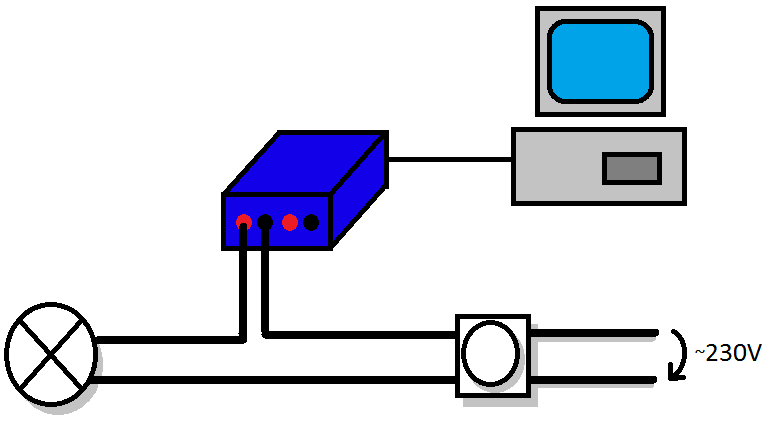
\includegraphics[width=1\textwidth]{Versuchsaufbau1.png}
\caption{Versuchsaubau um angeschnittenen Strom zu messen}
\end{figure}
\subsection{Versuchsdurchführung}
\subsubsection{Spektrum mit Fensterung}
An dem Phasenanschnittdimmer wird ein Zündwinkel eingestellt. Dieser kann aber nicht am Dimmer bestimmt werden, da eine Skala fehlt. Statt dessen wird das Phasenangeschnittene Signal zunächst mit dem Ossziloskop gemessen. Dabei wird die Zeitdifferenz zwischen dem Nulldurchgang und Zündmoment gemessen. Anschließend wird das Signal auch mit dem Sensorknoten abgetastet.\\ Um den Leckeffekt von vornerein zu umgehen, wird als Messdauer ein ganzzahliges vielfaches der Signalperiode (20ms) gewählt.\\ Die Abtastfrequenz muss wie folgt gewählt werden. Die 3dB-Grenzfrequenz des Allaisingfilters liegt bei 2,05kHz, die Auflösung des ADUs beträgt 10Bit und der Eingangsspannungsbereich beträgt 14V.\\
\begin{align}
U_{LSB} = \frac{14V}{2^{10}-1} = 0,01368V 
\end{align} 
Nun kann die benötigte Dämpfung, um Allaising zu verhindern, berechnet werden.\\
\begin{align}
D = 20 \cdot log_{10}(\frac{14V}{U_{LSB}}) = 60dB
\end{align} 
Der Filter ist ein Filter 8.Ordnung und besitzt eine Steilheit von 160dB/Dekade. Es wird abgeschätzt, dass der Filter ab ca.7kHz um über 60dB dämpft. Daher muss die Abtastfrequenz mindestens 14kHz betragen.
\subsubsection{Auswirkungen des Fensters}
Es werden nun nacheinander Rechteck-, Hanning- und Blackmanfenster über das Signal gelegt. Die Längen der Fenster sind absichtlich so gewählt, dass es zum leckeffekt kommt. Es wird nun untersucht, wie sich die unterschiedlichen Fenster auf den Leckeffekt auswirken. 
\subsubsection{Qualität der Netzspannung}
Nun soll die Qualität der Netzspannung überprüft werden. Theoretisch beträgt die Netzspannung 230V bei 50Hz. Allerdings können auf der Grundwelle zusätzlich zu den 50Hz weitere Oberwellen vorhanden sein. Der Anteil dieser Oberwellen an der Versorgungsspannung darf nicht über $8\%$ liegen.\\Für diesen Versuch wird die Netzspannung an den Spannungswandler der Blauenbox angelegt. Nun kann mit dem Sensorknoten die Netzspannung gemessen werden. Der Spannungswandler setzt die Eingangsspannung um den Faktor 56,6 herrab. Um die Netzspannung zu bestimmen, muss der Messwert mit 56,6 multipliziert werden.
\begin{figure}[htb]
\centering
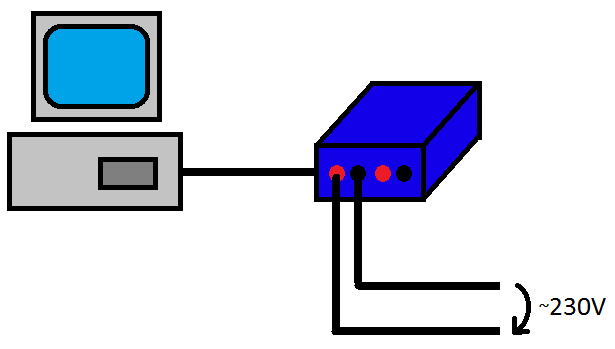
\includegraphics[width=1\textwidth]{Versuchsaufbau2.png}
\caption{Versuchsaubau um Netzqualität zu messen}
\end{figure}
\subsection{Versuchsauswertung}
\subsubsection{Spektrum mit Fensterung}
Von dem aufgezeichenteten Verlauf des phasenangeschnittetenen Stroms soll das Frequenz- und das Phasenspektrum bestimmt werden. Bei der Auswertung ist darauf zu achten, dass das Spektrum nicht durch schlechte Wahl des Fensters und der Messdauer verfälscht wird.\\ Der Leckeffekt wird umgangen, indem die Messdauer ein ganzzahliges Vielfaches der Signalperiode beträgt. Die Messdauer wurde zu 40ms gewählt. Dies ist die zweifache Periode der Grundwelle.\\ Es sollen pro Periode 300 Samples aufgenommen werden, um den Verlauf des Signals gut zu verfolgen. Daraus ergibt sich folgende Samplerate.
\begin{align}
f_{Samplerate} = \frac{T_{Messdauer}}{N_{Messwerte}} = 15000Hz
\end{align} 
Die Mindestsamplerate beträgt 14kHz. Eine Abtastrate von 15kHz ist also ausreichen um das Signal alliasingfrei abzutasten.\\Als Fenster wird das Hanningfenster gewählt. Es hat ein breites Hauptmaxima. Dadurch wird der Leckeffekt stark unterdrückt. Allerdings ist es nicht sehr frequenzselektiv. Dies ist in diesem Fall aber nicht von großer Bedeutung, da laut der Simulation (Vorbereitungsaufgaben Termin 3) die wichtigen Frequenzanteile ca. 50Hz von einander entfernt sind.\\ Das Spektrum des Signals müsste nun halbwegs vom Leckeffekt befreit sein. Allerdings sind die Amplituden durch den Frequenzgang des Antiallaisingfilters und durch die Fensterfunktion verzerrt. Um den Frequenzgang des Filters zu kompensieren, wird das Spektrum mit dem inversen Frequenzgang korrigiert. Die Verzerrung durch das Fenster kann korrigiert werden, indem das Spektrum durch die Summe des Fensters geteilt wird.\\
\begin{figure}[htb]
\centering
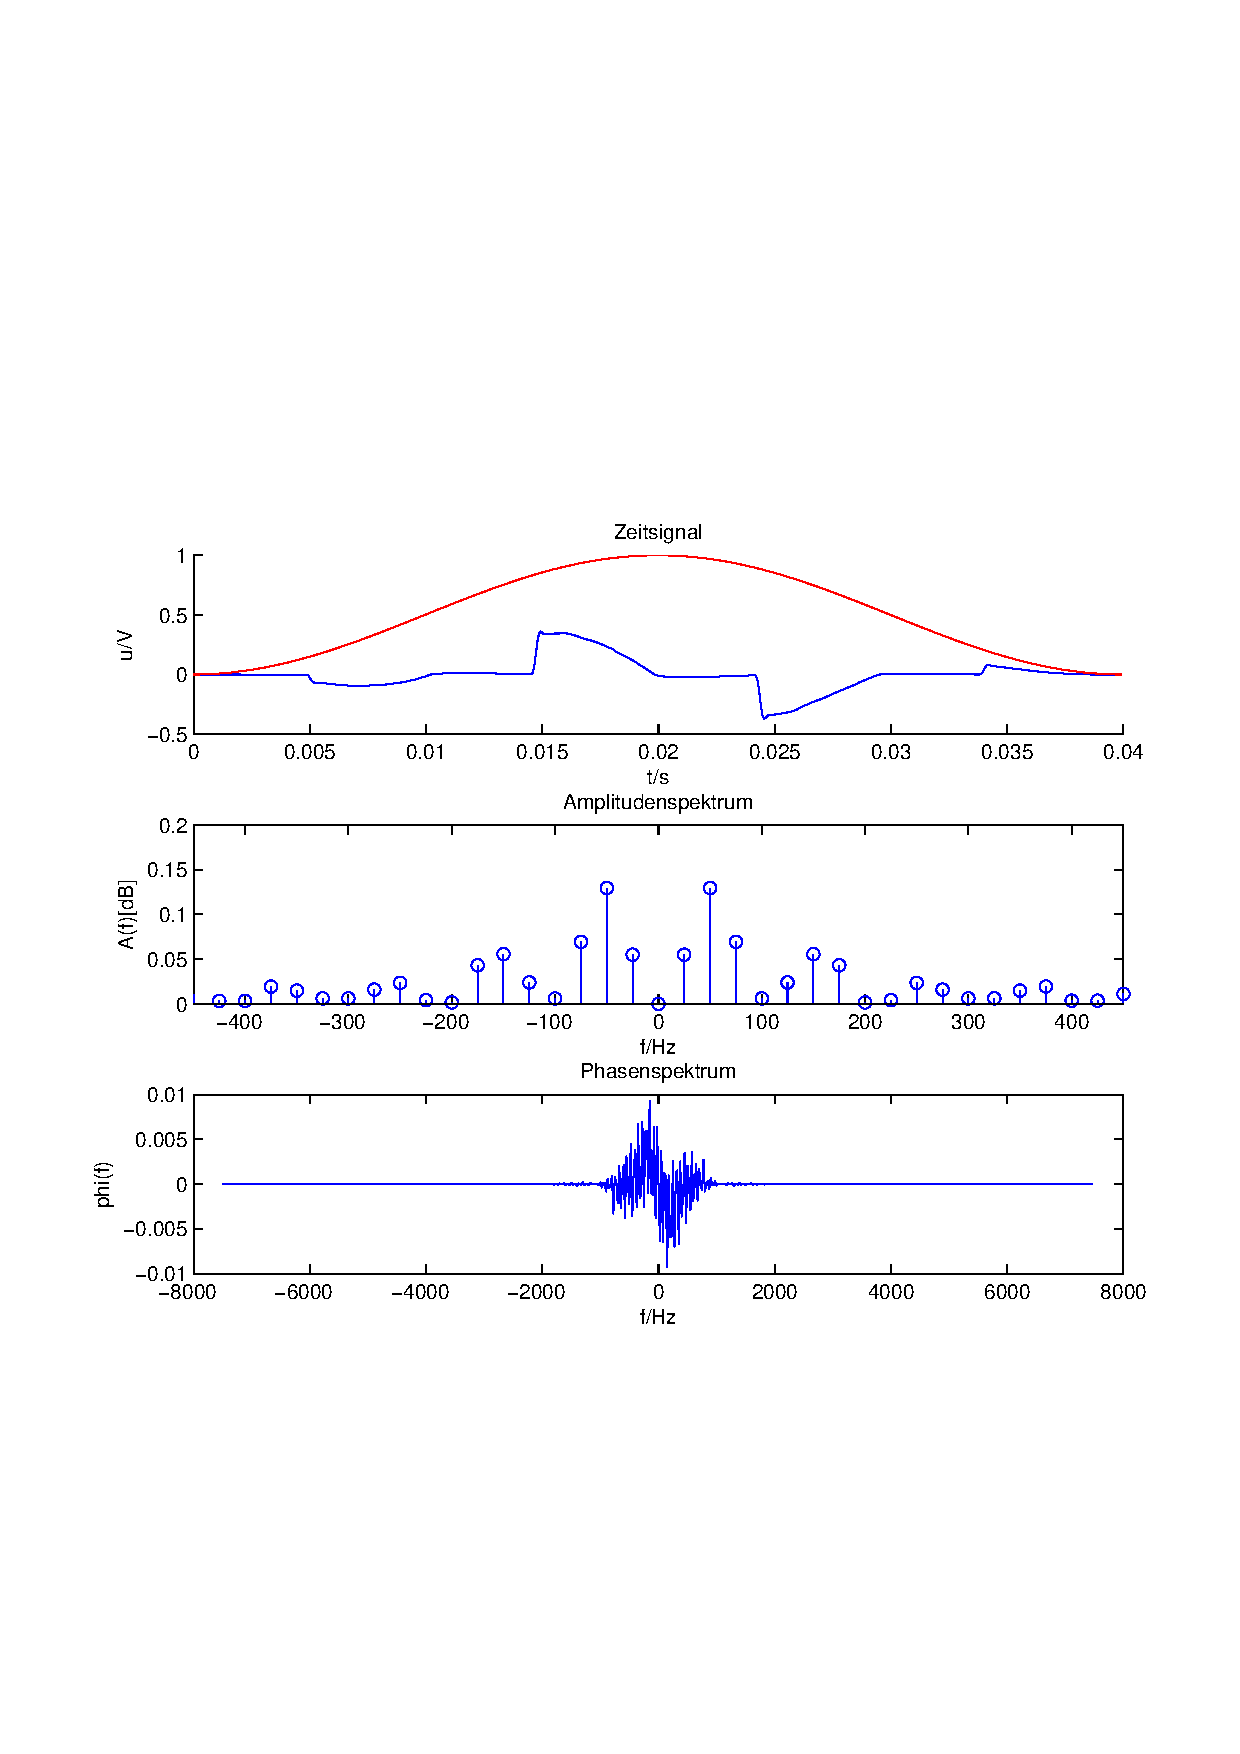
\includegraphics[width=1\textwidth]{Phasenanschnittsmessungmithanningfenster.pdf}
\caption{Spektrum des angeschnittenen Sinus mit Hanningfenster}
\end{figure} 
Im Vergleich mit der Simulation aus den Vorbereitungsaufgaben von Termin 3, fällt auf, dass die klaren Spektrallinien stark verlaufen sind. Der Leckeffekt ist also trotz Fenster aufgetreten. Dies liegt daran, dass alle Fensterfunktionen, außer dem Rechteckfenster, das Amplitudenspektrum verlaufen lassen.\\ Da das Fenster relativ genau 2 Perioden des Messsignals beträgt, kann mit dem Rechteckfenster ein wesendlich genaueres Spektrum bestimmt werden.\\ 
\begin{figure}[htb]
\centering
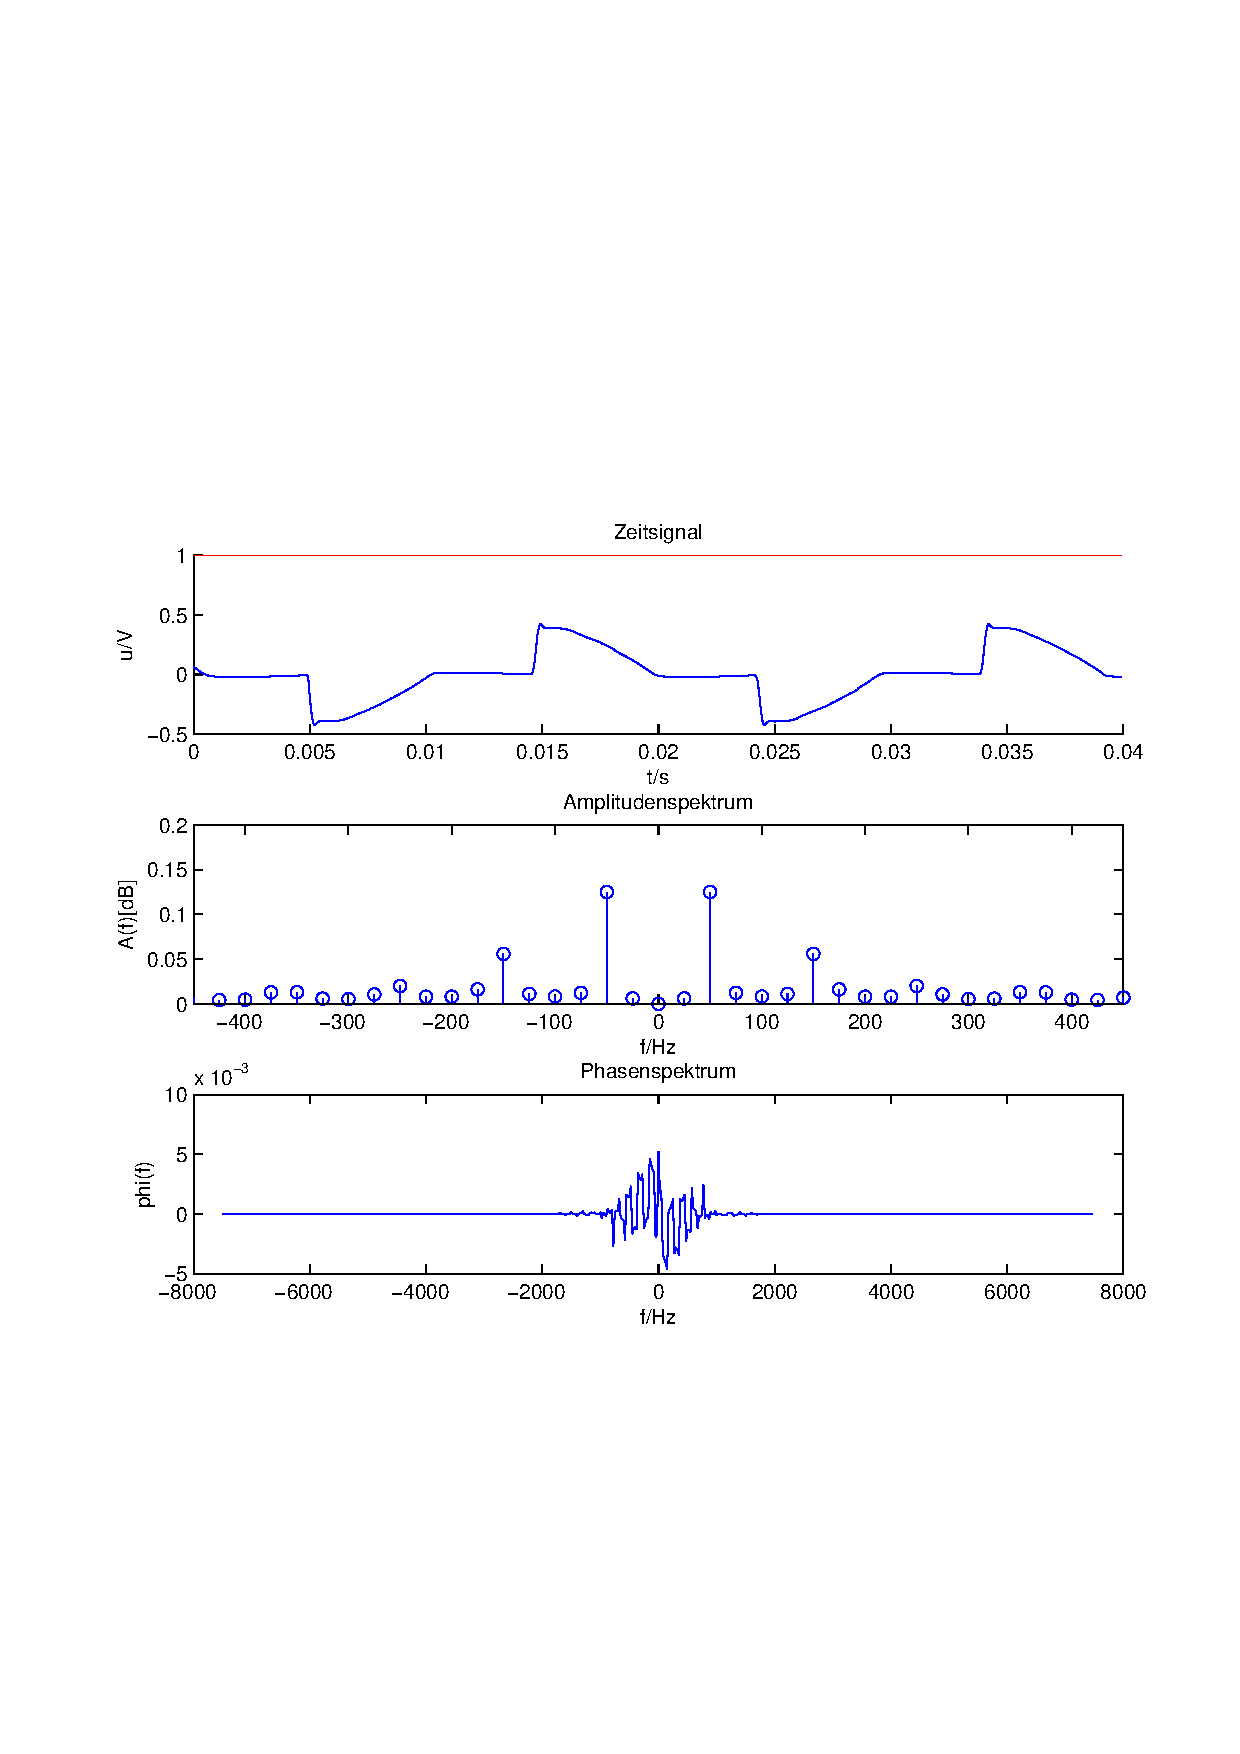
\includegraphics[width=1\textwidth]{Phasenanschnittsmessungmitrechteckfenster.pdf}
\caption{Spektrum des angeschnittenen Sinus mit Hanningfenster}
\end{figure} 
Wenn das zu messende Signal eine konstante, bekannte Periode besitzt, ist es vorteilhaft ein Rechteckfenster zu verwenden. Das Signal kann seine form dabei beliebig verändern. Sollte die Periode des Signals nicht konstant sein ist es aber besser eine Fensterfunktion zu verwenden um den Leckeffekt zumindest zu verringern.
\subsubsection{Netzqualität bestimmen}
Die Qualität der Netzspannung wird mit folgender Formel bestimmt.
\begin{align}
THD = \frac{\sqrt{{U_2}^2+{U_3}^2+ \cdot + {U_N}^2}}{U_1}
\end{align}   
Es wird die geometrische Summe aller Oberwellen gebildet und durch die Grundwelle geteilt.
Dabei ergab sich ein Anteil der Oberwellen von $3,32\%$ an dem gesamten Signal. Dieser Wert liegt unter den maximal zulässigen $8\%$.\\ Es ist zu beachten, das nicht alle Oberwellen gemessen wurden und dadurch auch nicht berücksichtigt wurden. Durch den Antiallaisingfilter wurden alle Frequenzen oberhalb von 7kHz ausgesperrt. Schnelle Störnadeln, die durch Schaltvorgänge entstehen und in einem Stromversorgungsnetz häufig vorkommen, werden daher nicht vollständig berücksichtigt. Daher wird THD tatsächlich etwas höher sein als der hier ermittelte Wert.
\begin{figure}[htb]
\centering
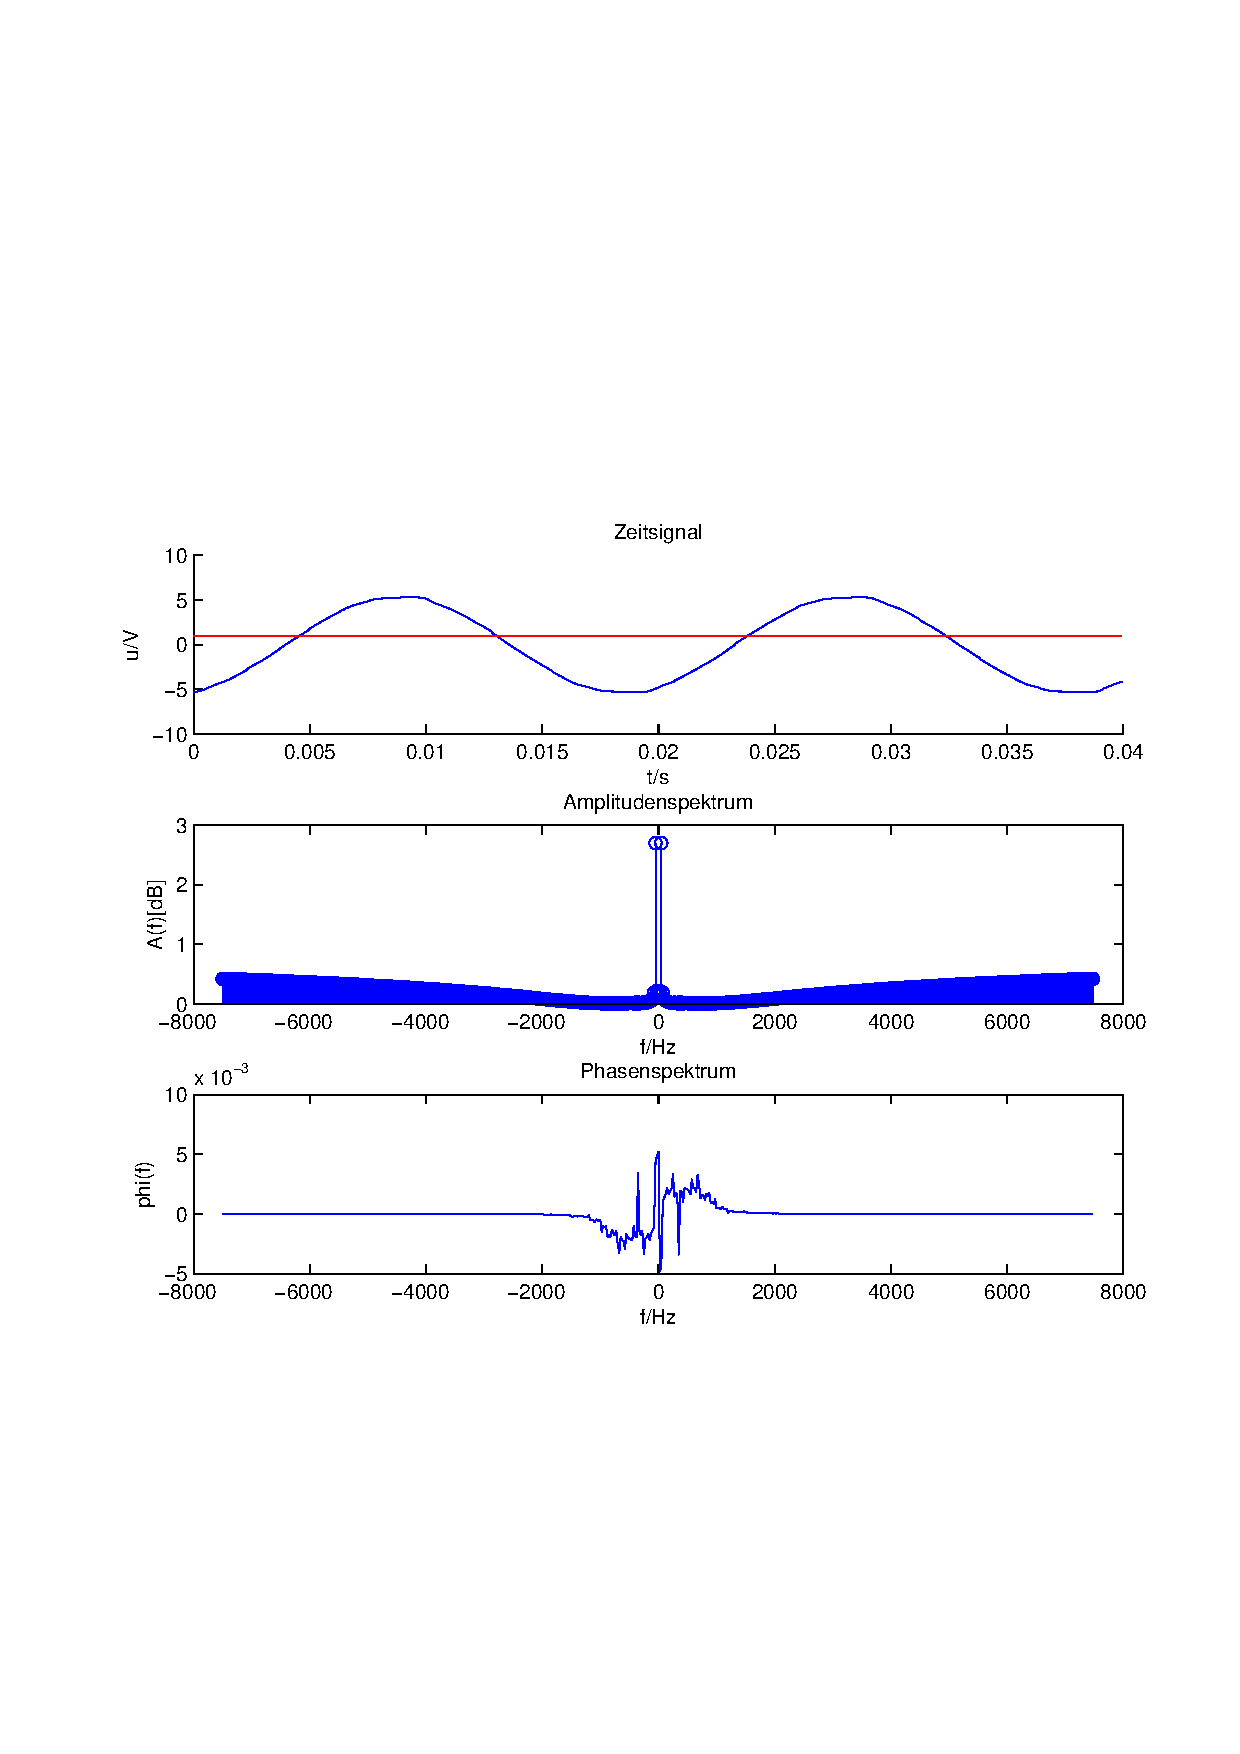
\includegraphics[width=1\textwidth]{OberwellenmessungspektrumTHD00332.pdf}
\caption{Spektrum des angeschnittenen Sinus mit Hanningfenster}
\end{figure}
\end{document}